
\documentclass[a4paper,11pt]{article}
\usepackage[a4paper, margin=8em]{geometry}

% usa i pacchetti per la scrittura in italiano
\usepackage[french,italian]{babel}
\usepackage[T1]{fontenc}
\usepackage[utf8]{inputenc}
\frenchspacing 

% usa i pacchetti per la formattazione matematica
\usepackage{amsmath, amssymb, amsthm, amsfonts}

% usa altri pacchetti
\usepackage{gensymb}
\usepackage{hyperref}
\usepackage{standalone}

% imposta il titolo
\title{Appunti Comunicazioni Numeriche}
\author{Luca Seggiani}
\date{2026}

% imposta lo stile
% usa helvetica
\usepackage[scaled]{helvet}
% usa palatino
\usepackage{palatino}
% usa un font monospazio guardabile
\usepackage{lmodern}

\renewcommand{\rmdefault}{ppl}
\renewcommand{\sfdefault}{phv}
\renewcommand{\ttdefault}{lmtt}

% disponi il titolo
\makeatletter
\renewcommand{\maketitle} {
	\begin{center} 
		\begin{minipage}[t]{.8\textwidth}
			\textsf{\huge\bfseries \@title} 
		\end{minipage}%
		\begin{minipage}[t]{.2\textwidth}
			\raggedleft \vspace{-1.65em}
			\textsf{\small \@author} \vfill
			\textsf{\small \@date}
		\end{minipage}
		\par
	\end{center}

	\thispagestyle{empty}
	\pagestyle{fancy}
}
\makeatother

% disponi teoremi
\usepackage{tcolorbox}
\newtcolorbox[auto counter, number within=section]{theorem}[2][]{%
	colback=blue!10, 
	colframe=blue!40!black, 
	sharp corners=northwest,
	fonttitle=\sffamily\bfseries, 
	title=~\thetcbcounter: #2, 
	#1
}

% disponi definizioni
\newtcolorbox[auto counter, number within=section]{definition}[2][]{%
	colback=red!10,
	colframe=red!40!black,
	sharp corners=northwest,
	fonttitle=\sffamily\bfseries,
	title=~\thetcbcounter: #2,
	#1
}

% U.D.M
\newcommand{\amp}{\ensuremath{\mathrm{A}}}
\newcommand{\volt}{\ensuremath{\mathrm{V}}}
\newcommand{\meter}{\ensuremath{\mathrm{m}}}
\newcommand{\second}{\ensuremath{\mathrm{s}}}
\newcommand{\farad}{\ensuremath{\mathrm{F}}}
\newcommand{\henry}{\ensuremath{\mathrm{H}}}
\newcommand{\siemens}{\ensuremath{\mathrm{S}}}

% circuiti
\usepackage{circuitikz}
\usetikzlibrary{babel}

% disegni
\usepackage{pgfplots}
\pgfplotsset{width=10cm,compat=1.9}

% disponi codice
\usepackage{listings}
\usepackage[table]{xcolor}

\definecolor{codegreen}{rgb}{0,0.6,0}
\definecolor{codegray}{rgb}{0.5,0.5,0.5}
\definecolor{codepurple}{rgb}{0.58,0,0.82}
\definecolor{backcolour}{rgb}{0.95,0.95,0.92}
\lstdefinestyle{codestyle}{
		backgroundcolor=\color{black!5}, 
		commentstyle=\color{codegreen},
		keywordstyle=\bfseries\color{magenta},
		numberstyle=\sffamily\tiny\color{black!60},
		stringstyle=\color{green!50!black},
		basicstyle=\ttfamily\footnotesize,
		breakatwhitespace=false,         
		breaklines=true,                 
		captionpos=b,                    
		keepspaces=true,                 
		numbers=left,                    
		numbersep=5pt,                  
		showspaces=false,                
		showstringspaces=false,
		showtabs=false,                  
		tabsize=2
}

\lstdefinestyle{shellstyle}{
		backgroundcolor=\color{black!5}, 
		basicstyle=\ttfamily\footnotesize\color{black}, 
		commentstyle=\color{black}, 
		keywordstyle=\color{black},
		numberstyle=\color{black!5},
		stringstyle=\color{black}, 
		showspaces=false,
		showstringspaces=false, 
		showtabs=false, 
		tabsize=2, 
		numbers=none, 
		breaklines=true
}

\lstdefinelanguage{javascript}{
	keywords={typeof, new, true, false, catch, function, return, null, catch, switch, var, if, in, while, do, else, case, break},
	keywordstyle=\color{blue}\bfseries,
	ndkeywords={class, export, boolean, throw, implements, import, this},
	ndkeywordstyle=\color{darkgray}\bfseries,
	identifierstyle=\color{black},
	sensitive=false,
	comment=[l]{//},
	morecomment=[s]{/*}{*/},
	commentstyle=\color{purple}\ttfamily,
	stringstyle=\color{red}\ttfamily,
	morestring=[b]',
	morestring=[b]"
}

% disponi sezioni
\usepackage{titlesec}

\titleformat{\section}
	{\sffamily\Large\bfseries} 
	{\thesection}{1em}{} 
\titleformat{\subsection}
	{\sffamily\large\bfseries}   
	{\thesubsection}{1em}{} 
\titleformat{\subsubsection}
	{\sffamily\normalsize\bfseries} 
	{\thesubsubsection}{1em}{}

% disponi alberi
\usepackage{forest}

\forestset{
	rectstyle/.style={
		for tree={rectangle,draw,font=\large\sffamily}
	},
	roundstyle/.style={
		for tree={circle,draw,font=\large}
	}
}

% disponi algoritmi
\usepackage{algorithm}
\usepackage{algorithmic}
\makeatletter
\renewcommand{\ALG@name}{Algoritmo}
\makeatother

% disponi numeri di pagina
\usepackage{fancyhdr}
\fancyhf{} 
\fancyfoot[L]{\sffamily{\thepage}}

\makeatletter
\fancyhead[L]{\raisebox{1ex}[0pt][0pt]{\sffamily{\@title \ \@date}}} 
\fancyhead[R]{\raisebox{1ex}[0pt][0pt]{\sffamily{\@author}}}
\makeatother

\begin{document}
% sezione (data)
\section{Lezione del 17-03-26}

% stili pagina
\thispagestyle{empty}
\pagestyle{fancy}

% testo
Nella scorsa lezione abbiamo descritto la trasformata di Fourier nella sua forma continua, in particolare esprimendo le equazioni di \textit{analisi} e di \textit{sintesi}. Vediamone adesso una forma numerica, che ci permette di trasformare segnali campionati arbitrati senza dover svolgere calcoli analitici.

\subsection{Trasformata di Fourier discreta}
Per "discretizzare" la trasformata di Fourier adottiamo il solito approccio alla discretizzazione di qualsiasi integrale, cioè preso:
$$
x(t) \rightarrow \int x(t) \, dt
$$
scegliamo un \textit{intervallo di campionamento} $\Delta t$:
$$
\Delta t, \quad f_s = \frac{1}{\Delta t}
$$
dove $f_s$ diventerà la nostra \textit{frequenza di campionamento}, e portiamo l'integrale alla sommatoria:
$$
\sum_{n=0}^{N - 1} x(n \Delta t) \cdot \Delta t
$$
su $N$ istanti temporali (si conta da $0$ a $N - 1$, totale $N$ campioni).

Applicando questo processo alla trasformata di Fourier (di cui ricordiamo l'equazione di \textit{analisi} in 6.1), otteniamo:
$$
X(k \Delta f) = \int_{-\infty}^{\infty} x(t) e^{-i 2 \pi k \Delta f t} \, dt \approx
\Delta t \sum_{n = 0}^{N - 1} x(n \Delta t) e^{- i 2 \pi k \Delta f n \Delta t}
$$
dove $\Delta t$, come abbiamo già detto, è l'intervallo di campionamento del segnale \textit{temporale}, mentre $\Delta f$ è l'intervallo di campionamento sullo spettro delle \textit{frequenze}. Spesso si prende:
$$
\Delta f = \frac{1}{N \Delta t}
$$
per avere la cosiddetta frequenza "normalizzata".

Notiamo che nella formula a destra, $n$ (indice temporale) e $k$ (indice nelle frequenze) possono essere scelti in maniera arbitraria:
\begin{itemize}
	\item Se calcoliamo la trasformata ad una certa frequenza $k \Delta f$, variamo $k$;
	\item Per calcolare la trasformata alla frequenza $k \Delta f$, prendiamo i contributi di tutti i possibili $n$ fra $0$ e $N - 1$.
\end{itemize}
Questo significherà che potremo portare l'operazione di trasformata di Fourier discreta in forma vettoriale (è di vettori di istanti temporali o di frequenza che si parla):
$$
\mathbf{X} =
\begin{pmatrix}
X\left( 0 \right) \\
\vdots \\
X\left( (K - 1) \Delta f \right)
\end{pmatrix} =
\Delta t \mathbf{F}
\begin{pmatrix}
x \left( 0 \right) \\
\vdots \\
x \left( (N - 1) \Delta t \right) \\
\end{pmatrix} =
\Delta t \mathbf{X} \mathbf{x}
$$
dove $K$ è la lunghezza del vettore di frequenze, $\mathbf{X}$ e $\mathbf{x}$ sono i vettori delle frequenze e dei campioni temporali rispettivamente, campionati nei punti $0, ..., K - 1$ e $0, ..., N - 1$.

La matrice $\mathbf{F}$ sarà invece quella degli operatori della trasformata di Fourier, cioè:
$$
\mathbf{F}_{kn} = e^{- i 2 \pi k \Delta f n \Delta t}
$$

Facciamo alcune considerazioni in termini di complessità. Abbiamo che:
\begin{itemize}
	\item $\mathbf{X}$ ha dimensione $K \times 1$;
	\item $\mathbf{x}$ ha dimensione $N \times 1$;
	\item $\mathbf{F}$ ha dimensione $K \times N$.
\end{itemize}
Questo significherà che il numero di operazioni necessarie è nell'ordine di:
$$
O(KN) \quad \left( O(N^2) \right)
$$
Da cui notiamo che, visto che spesso prendiamo $K = N$, cioè tanti "bucket" (campioni) frequenziali quanti sono i campioni temporali, avremo che la complessità complessivamente sarà data da $O(N^2)$. Questo è chiaramente poco ottimale, in quanto spesso si vogliono trasformare segnali ad alte frequenze di campionamento. Abbiamo quindi bisogno di un approccio migliore.

\subsubsection{Trasformata di Fourier discreta veloce}
Un algoritmo più veloce per calcolare la trasformata di Fourier discreta è ad esempio quello che è stato usato per disegnare i grafici nella lezione precedente. Lo script usato per la generazione del grafico era basato sull'implementazione dell'algoritmo \textbf{FFT} (\textit{Fast Fourier Transform}, in italiano appunto \textit{trasformata di Fourier discreta veloce}), in particolare nella versione di \textit{Cooley}-\textit{Tukey}. Se ne trova una versione nella directory \texttt{code/python} di questi appunti.

L'algoritmo della trasformata di Fourier discreta veloce si basa sull'osservazione che negli $N^2$ passaggi dove combiniamo ogni valore di $k$ con ogni valore di $n$ si svolgono diverse volte calcoli che potrebbero essere fatti una volta sola, e quindi memoizzati. 

Presentiamo quindi una versione specifica della trasformata di Fourier veloce, data dall'algoritmo di \textit{Cooley}-\textit{Tukey}, in versione a \textit{radice 2}.

La forma della trasformata discreta che adottiamo è quella a frequenza normalizzata, cioè preso $\Delta f = \frac{1}{N \Delta t}$:
$$
X_k = \sum_{n=0}^{N-1} x_n e^{- \frac{2\pi i}{N} nk}
$$

L'intuizione sarà quindi quella di dividere la DFT di dimensione $N$ in due DFT "interlacciate" di dimensione $\frac{N}{2}$, in modo da poter risparmiare calcoli ripetuti adottando un approccio \textit{divide et impera}. Dal punto di vista algebrico, separiamo gli indici pari e dispari:
$$
X_k =
\sum_{m=0}^{N/2-1} x_{2m} e^{- \frac{2\pi i}{N}(2m)k}
+
\sum_{m=0}^{N/2-1} x_{2m+1} e^{- \frac{2\pi i}{N}(2m+1)k}.
$$
ed estraiamo uno degli esponenziali a destra:
$$
X_k =
\sum_{m=0}^{N/2-1} x_{2m} e^{- \frac{2\pi i}{N/2} mk}
+
e^{- \frac{2\pi i}{N} k}
\sum_{m=0}^{N/2-1} x_{2m+1} e^{- \frac{2\pi i}{N/2} mk}.
$$

Possiamo quindi definire le due forme, che troviamo sostanzialmente equivalenti:
$$
E_k = \sum_{m=0}^{N/2-1} x_{2m} e^{- \frac{2\pi i}{N/2} mk}, \quad
O_k = \sum_{m=0}^{N/2-1} x_{2m+1} e^{- \frac{2\pi i}{N/2} mk}.
$$
dove $E_k$ è la trasformata di Fourier calcolata sui campioni "dimezzati" pari, e $O_k$ è la sua analoga calcolata sui campioni dispari. Potremo quindi scrivere semplicemente: 
$$
X_k = E_k + e^{- \frac{2\pi i}{N} k} O_k,
$$
cioè abbiamo un modo per riportare i risultati intermedi (calcolati su finestre dimezzate) nel risultato finale. Notiamo che la sfortuna di questo approccio è che vale solo per $n = 0, ..., \frac{N}{2} - 1$ compreso. Per calcolare il resto dei campioni frequenziali (da $n = \frac{N}{2}, ..., N - 1$), sfruttiamo le proprietà di periodicità dell'esponenziale:
$$
X_{k + N/2} = E_k - e^{- \frac{2\pi i}{N} k} O_k.
$$

Notiamo che i fattori:
$$
e^{- \frac{2\pi i}{N} k}, \quad -e^{- \frac{2\pi i}{N} k}
$$
vengono detti \textit{fattori di twiddle}, ed è solitamente utile precalcolarli.

Questo costituisce il nucleo dell'algoritmo FFT radice 2. Possiamo applicare l'operazione di divisione in 2 finestre "dimezzate" un numero arbitrario di volte (anche se in casi reali a conviene fermarsi prima), scendendo ricorsivamente fino al caso di dimensione 1 (dove restituiamo l'unico campione dato).

\newpage

Questo, in codice Python, ha il seguente (semplicissimo) aspetto:
\begin{lstlisting}[language=python, style=codestyle]	
def fft(x):
    ln = len(x)
    hln = ln // 2

    if ln == 1:
        # base case 
        return x
    else:
        # calculate even/odd FFTs
        even = fft(x[0::2])
        odd  = fft(x[1::2])

        # merge even/odd FFTS in result
        res = [None] * ln 
        for k in range(0, hln):
            twid = cmath.exp(-2j * math.pi * k / ln)
            X[k]       = even[k] + twid * odd[k] 
            X[k + hln] = even[k] - twid * odd[k] 
        return res
\end{lstlisting}

\subsubsection{Antitrasformata di Fourier discreta}
L'antitrasformata discreta di Fourier si calcola in maniera completamente duale alla trasformata. Ad esempio, prendendo la forma matriciale di prima, abbiamo che si passa alla matrice \textit{hermitiana}:
$$
\mathbf{x} = \Delta f \mathbf{F}^H \mathbf{X}
$$
con $\mathbf{x}$, $\mathbf{F}$ e $\mathbf{X}$ presi come prima. 

Anche la antitrasformata discreta ha un algoritmo ottimizzato, con intuizione e pseudocodice simile al precedente, che non riportiamo per semplicità. Tale algoritmo prende il nome di \textbf{IFFT} (\textit{Inverse Fast Fourier Transform}).

\subsection{Teoremi sulla trasformata di Fourier}
Veniamo a vedere alcuni teoremi relativi alla trasformata di Fourier.

\begin{enumerate}
\item \begin{theorem}{Linearità della trasformata di Fourier}
Vale che:
$$
x(t) = \alpha_1 x_1(t) + \alpha_2 x_2(t) \implies X(f) = \alpha_1 X_1(f) + \alpha_2 X_2(f)
$$
\end{theorem}
Questo viene direttamente dalla forma dell'equazione di analisi:
$$
X(f) = \int_{-\infty}^{\infty} \alpha_1 x_1(t) e^{-i 2 \pi  f t} \, dt + \int_{-\infty}^{\infty} \alpha_2 x_2(t) e^{-i 2 \pi  f t} \, dt
$$
e applicando la linearità dell'operatore integrale (possiamo estrarre gli $\alpha_i$), per cui:
$$
X(f) = \alpha_1 X_1(f) + \alpha_2 X_2(f)
$$
che è la tesi. \hfill $\square$

\item \begin{theorem}{Dualità della trasformata di Fourier}
Vale che:
$$
x(t) \rightarrow X(f) \implies X(t) \rightarrow x(-f)
$$
\end{theorem}
Questo viene in qualche modo dalle osservazioni sulla simmetria fatte in 6.1.1. In particolare, scambiando $t$ ed $f$ nell'equazione di sintesi, si ha:
$$
x(f) = \int_{-\infty}^{\infty} X(t) e^{i 2 \pi t f} \, dt
$$
per cui notiamo che dobbiamo scambiare $f$ con $-f$ per ottenere:
$$
x(-f) = \int_{-\infty}^{\infty} X(t) e^{-i 2 \pi f t} \, dt
$$
che è la tesi. \hfill $\square$

Applicando questo teorema, ad esempio, ala funzione rettangolare (vista sempre in 6.1.1), otteniamo:
$$
x(t) = \mathrm{rect} \left( \frac{t}{\tau} \right) \rightarrow \tau \mathrm{sinc} (f \tau) \implies \tau \mathrm{sinc} (t \tau) \rightarrow \mathrm{rect} \left(\frac{f}{\tau}\right) 
$$
mentre applicandolo alla funzione esponenziale monolatera si ha:
$$
x(t) = e^{-\frac{t}{\tau}} u(t) \rightarrow \frac{\tau}{1 + i 2 \pi f \tau} \implies \frac{\tau}{1 + i 2 \pi t \tau} \rightarrow e^{\frac{f}{\tau}} u(-f)
$$
Notiamo una particolarità di questo ultimo spettro è che non è simmetrico: questo è reso possibile dal fatto che il segnale considerato, cioè:
$$
X(t) = \frac{\tau}{1 + i 2 \pi t \tau}
$$
è \textit{complesso} $\in \mathbb{C}$ (quindi non ha ipotesi di simmetria).

\item \begin{theorem}{Ritardo della trasformata di Fourier}
Vale che:
$$
y(t) = x(t - t_0) \implies Y(f) = X(f) e^{-i 2 \pi f t_0}
$$
\end{theorem}

Cioè un ritardo temporale introduce una variazione di fase che cambia linearmente con la frequenza, ma non cambia lo spettro di ampiezza. Diciamo linearmente, in quanto dobbiamo ricordare che:
$$
|Y(f)| = |X(f)|, \quad \mathrm{arg} \left( Y(f) \right) = \mathrm{arg} \left( X(f) \right) - 2 \pi f t_0
$$

Questo si dimostra dall'equazione di analisi:
$$
X(f) = \int_{-\infty}^{\infty} x(t - t_0) e^{-i 2 \pi f t} \, dt
$$
Ponendo il cambio di variabile $\alpha = t - t_0$, si ottiene:
$$
X(f) = \int_{-\infty}^{\infty} x(\alpha) e^{-i 2 \pi f \alpha + t_0} \, d \alpha = e^{-i 2 \pi f t_0} \int_{-\infty}^{\infty} x(\alpha) e^{-i 2 \pi f \alpha} \, d \alpha
$$
che è la tesi. \hfill $\square$

\item \begin{theorem}{Teorema della modulazione}
Vale che:
$$
x(t) \cos(2 \pi f_0 t) \rightarrow \frac{X(f - f_0) + X(f + f_0)}{2}
$$
\end{theorem}

Il teorema della modulazione è utile, appunto, nel contesto della \textit{modulazione} dei segnali in fase di preparazione alla trasmissione sul mezzo. Nell'analisi del trasmettitore fatta in 1.2, siamo nel componente \textit{modulator}, che prende il segnale digitale preso dal channel encoder, e lo transforma in una forma d’onda adatta a essere trasmessa sul mezzo.

Ad esempio, nelle radio vecchio stile, la manopola del sintonizzatore variava la capacità di un circuito che faceva da filtro passa-banda, cioè isolava una sola regione dello spettro, dove era contenuto il segnale da ricevere (modulato). Oggi nella radio vale un processo simile, ma svolto attraverso transistor o in digitale.

Il fatto che si possano modulare segnali a diverse frequenze, assieme al teorema 7.1 (di \textit{linearità}), significa che possiamo piazzare più segnali temporali a frequenze diverse dello spettro (dello spettro radio, ad esempio). Questo permette a più dispositivi di usare lo stesso mezzo di trasmissione, dividendolo in diverse porzioni di frequenze. Chiaramente, se vogliamo riportarci al segnale in dominio tempo originale, dobbiamo prevedere un passaggio di \textit{filtraggio} simile a quello della radio a capacità visto sopra. Fra l'altro, questo è il processo dell'accesso multiplo in \textbf{FDMA} (\textit{Frequency Division Multiple Access}) visto in 1.2.4.

\begin{center}
	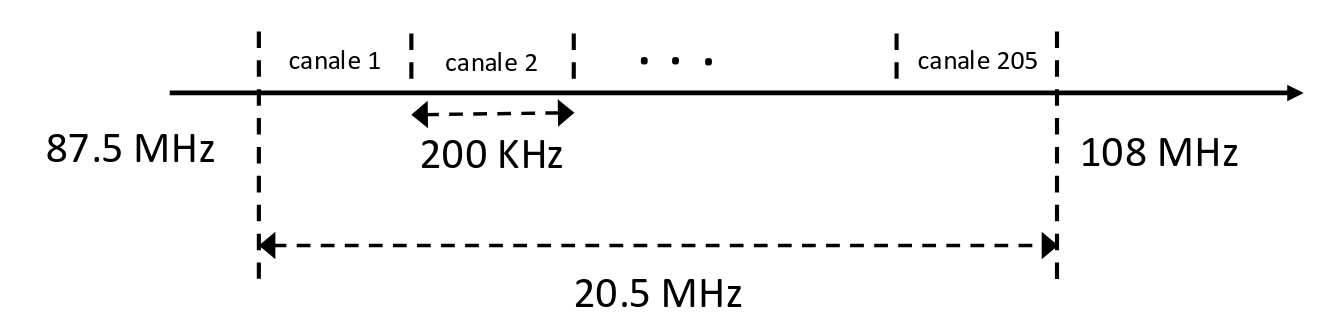
\includegraphics[scale=0.25]{../figures/spec_spec.png}
\end{center}

Inoltre, perché la modulazione abbia l'effetto desiderato, dobbiamo scegliere frequenze di modulazione $f_0$ molto più grandi di quelle del segnale originale $f$, in modo che $f + f_0$ ci porti a destra nelo spettro di frequenze (nella regione di frequenze che allochiamo al segnale) e $f - f_0$ finisca nella regione $f < 0$ (e non crei due "lobi" attorno alla $f$ originale).

Dimostriamo quindi il teorema. Il risultato ottenuto si ha dall'equazione di analisi applicata all'espressione data:
$$
X(f) = \int_{-\infty}^{\infty} x(t) \cos(2 \pi f_0 t) e^{-i 2 \pi f t} \, dt
$$
e prendendo il coseno nella forma esponenziale data dalle equazioni di Eulero:
$$
\cos(\alpha) = \frac{e^{i\alpha} + e ^{-i\alpha}}{2}
$$
da cui:
$$
X(f) = \int_{-\infty}^{\infty} x(t) \frac{e^{i 2\pi f_0 t} + e^{-i 2 \pi f_0 t}}{2} e^{-i 2 \pi f t} \, dt 
$$
$$
= \frac{1}{2} \int_{-\infty}^{\infty} x(t) e^{-i 2 \pi (f - f_0) t} \, dt + \frac{1}{2} \int_{-\infty}^{\infty} x(t) e^{-i 2 \pi (f + f_0) t} \, dt = \frac{X(f - f_0) + X(f + f_0)}{2}
$$
che è la tesi. \hfill $\square$

\end{enumerate}


\end{document}
